\section{Espacios de Probabilidad}
\subsection{Instroducción y definiciones de probabilidad}
Disitnguen varios tipos de experimentos:
\begin{itemize}
	\item Experimentos deterministas.
	\item Experimentos aleatorios: proporcionan resultados distintos aunque se realicen bajo las mismas pruebas.
	\item Experimento pseudoaleatorios.
\end{itemize}
La Teoría de la Probabilidad estuida los experimentos aleatorios.
\begin{itemize}[label=\color{red}\textbullet, leftmargin=*]
	\item \color{lightblue}Definición (Laplace)
\end{itemize}
Si todos los resultados del experimentos son equiprobables, se define \[ P(A)=P(\text{"Ocurre $A$"})=\dfrac{\text{nº de casos favorables $A$}}{\text{nº de casos posibles}} \]
\Ej
\[ P(\text{"Sacar nº par al lanzar un dado"})\longrightarrow\dfrac{3}{6}=\dfrac{1}{2} \]
\begin{itemize}[label=\color{red}\textbullet, leftmargin=*]
	\item \color{lightblue}Definición (Teoría de Von Misses)
\end{itemize}
Vale en el caso de experimentos con resultados \lb{no} equiprobables. \[ P(A)=\lim_{n\to\infty}\dfrac{\text{Nº de veces que obtengo $A$}}{n}=\lim_{n\to\infty}f_r(A)\lb{ (\text{frecuencia relativa})} \]donde $n=$"nº de veces que repito el experimento".
\begin{itemize}[label=$-$]
	\item Inconveniente: no siempre puedo calcular el límite o repetir el experimento.
\end{itemize}

\begin{itemize}[label=\color{red}\textbullet, leftmargin=*]
	\item \color{lightblue}Definición (Axiomática de Kolmogorov)
\end{itemize}

\begin{wrapfigure}[2]{r}{0.5\textwidth}
	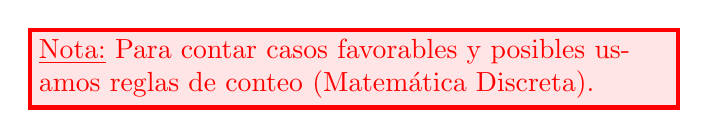
\begin{tikzpicture}
		\node[red, draw=red, fill=red!10, text width=8cm, line width=1.5] {\underline{Nota:} Para contar casos favorables y posibles usamos reglas de conteo (Matemática Discreta).};
	\end{tikzpicture}
\end{wrapfigure}

Es la que se usa en Teoría de la Probabilidad y permite construir una teoría consistente.
\begin{itemize}[label=\color{red}\textbullet, leftmargin=*]
	\item \color{lightblue}Espacios de probabilidad y $\sigma$-álgebras
\end{itemize}
Consideraremos un experimento aleatorio.
\begin{itemize}[label=\color{red}\textbullet, leftmargin=*]
	\item \color{lightblue}Definición
\end{itemize}
\begin{itemize}[label=$-$]
	\item Llamaremos \lb{espacio muestral}, $\Omega$, al conjunto de todos los resultados individuales posibles del experimento aleatorio.
	\item Llamaremos \lb{suceso elemental} a cada uno de los resultados individuales.
	\item Llamaremos \lb{suceso} a cualquier subconjunto de $\Omega$ (agrupaciones de resultados.)
\end{itemize}
Denotaremos por $\mathcal{S}$ al conjunto de todos los sucesos sobre los que queremos calcular su probabilidad. Observar que $\mathcal{S}\subseteq P(\Omega)$.

Los sucesos suelen denotar por letras mayúsculas $A,B,C,\dots$\\
\Ej\\
Experimento aleatorio: "Observar el resultado al lanzar un dado".
\begin{itemize}[label=$-$]
	\item $\Omega=\{1,2,3,4,5,6\}$
	\item Sucesos elementales: $\left\{\{1\},\{2\},\dots,\{6\}\right\}$
	\item Algunos sucesos:
	
	$A=$"Obtener número par"$=\{2,4,6\}\subseteq\Omega\longrightarrow$ un suceso.\\
	$B=$"Obtener valor $\le3=\{1,2,3\}\subseteq\Omega\longrightarrow$ un suceso.
\end{itemize}
Operaciones con sucesos:
\begin{multicols}{3}
	\begin{itemize}[label=$-$]
		\item $A\cup B$
		\item $A\cap B$
		\item $A^c=\overline{A}=\Omega-A$
		\item $A+B=A\cap B^c$
		\item $A\triangle B=(A-B)\cup(B-A)$
\end{itemize}
\end{multicols}
\begin{itemize}[label=\color{red}\textbullet, leftmargin=*]
	\item \color{lightblue}Propiedades
\end{itemize}
\begin{itemize}[label=$-$]
	\item $A\cup(B\cap C)=(A\cup B)\cap(A\cup C)$
	\item $A\cap(B\cup C)=(A\cap B)\cup(A\cap C)$
	\item $A\cup A^c=\Omega$
	\item Leyes de Morgan:
	\begin{itemize}[label=$-$]
		\item $(A\cup B)^c=A^c\cap B^c$
		\item $(A\cap B)^c=A^c\cup B^c$
	\end{itemize}
\end{itemize}
\begin{itemize}[label=\color{red}\textbullet, leftmargin=*]
	\item \color{lightblue}Definición Axiomática de Kolmogorov
\end{itemize}
Llamaremos \lb{espacio de probabilidad} a una terna $(\Omega, \mathcal{S}, P)$ formada por un conjunto $\Omega$, un conjunto $\mathcal{S}\subseteq P(\Omega)$ y una función de posibilidad \begin{align*}
	P:&\mathcal{S}\longrightarrow\R\\
	&A\longrightarrow P(A)
\end{align*}
Verificando los siguientes axiomas:
\begin{enumerate}[label=Ax\arabic*)]
	\item $\Omega\in\mathcal{S}$
	\item Si $A\in\mathcal{S}$, entonces $A^c\in\mathcal{S}$
	\item Si $A_1,A_2,\dots\in\mathcal{S}$, entonces $A_1\cup A_2\cup \cdots\in\mathcal{S}$
	\item $P(\Omega)=1$
	\item $P(A)\ge0\:\forall A\in\mathcal{S}$
	\item Si $A_1,A_2,\dots\in\mathcal{S}$ sucesos dispuestos dos a dos $A_i\cap A_j=\varnothing\:\forall i\neq0$, entonces $P(A_1\cup A_2\cup\dots)=P(A_1)+P_(A_2)+\cdots$
\end{enumerate}
\begin{itemize}[label=\color{red}\textbullet, leftmargin=*]
	\item \color{lightblue}Definición
\end{itemize}
Si $\Omega$ es un conjunto y $\mathcal{S}$ cumples los axiomas 1, 2 y 3 se dice que $\mathcal{S}$ es una $\sigma$-álgebra.\\
La $\sigma$-álgebra generada por los intervalos abierto de $\R$ (de $\R^n$) se llama $\sigma$-álgebra de Borel.

\Ej

Experimento aleatorio con $\Omega$ finito. $\Omega=\{w_1,w_2,\dots,w_n\}$\\
$\mathcal{S}=P(\Omega)$ es una $\sigma$-álgebra (porque $P(\Omega)$ siempre es $\sigma$-álgebra).\begin{align*}
	P:&\mathcal{S}\longrightarrow\R\\
	&A\longrightarrow P(A)=\dfrac{\text{casos favorables a $A$}}{\text{casos posibles experimento}}=\dfrac{\mathrm{cardinal}(A)}{n}=\dfrac{|A|}{n}
\end{align*}Entonces $(\Omega,\mathcal{S},P)$ es un espacio de probabilidad.
\begin{itemize}[label=\color{red}\textbullet, leftmargin=*]
	\item \color{lightblue}Demostración
\end{itemize}
Ax1,2,3,4 y 5 triviales. Como $\Omega$ es finito bastaría probar Ax6 para el caso de dos sucesos. Sean $A$ y $B$ sucesos disjuntos $A\cap B=\varnothing$.

¿$P(A\cup B)=P(A)+P(B)$?

\[ P(A\cup B)=\dfrac{|A\cup B|}{n}=\lb{\left\{\text{porque }A\cap B=\varnothing\right\}}=\dfrac{|A|+|B|}{n}=\dfrac{|A|}{n}+\dfrac{|B|}{n}=P(A)+P(B) \]
\subsection{Propiedades de las $\sigma$-álgebras y de la función probabilidad}
\begin{itemize}[label=\color{red}\textbullet, leftmargin=*]
	\item \color{lightblue}Propiedades
\end{itemize}
Sea $\mathcal{S}$ una $\sigma$-álgebra de $\Omega$ entonces:
\begin{enumerate}[label=\color{lightblue}\arabic*)]
	\item $\varnothing\in\mathcal{S}$: Por Ax1 sabemos que $\Omega\in\mathcal{S}$ y por Ax2 sabemos que $\Omega^c=\varnothing\in\mathcal{S}$.
	\item Si $A$ y $B\in\mathcal{S}\longrightarrow A\cup B\in\mathcal{S}$: Aplico el Ax3 con los sucesos $A_1=A,A_2=B,A_3=A_4=\cdots=\varnothing$.
	\item Si $A,B\in\mathcal{S}\longrightarrow A\cap B\in\mathcal{S}$: Sbamos que $\lbb{A^c,B^c\in\mathcal{S}}{Ax2}$ y también $\lbb{A^c\cup B^c}{\text{Prop. }2}$
	\item $A,B\in\mathcal{S}\longrightarrow A-B\in\mathcal{S}:A-B=A\cap B^c\in\mathcal{S}$
	\item $A,B\in\mathcal{S}\longrightarrow A\triangle B\in\mathcal{S}:A\triangle B=(A-B)\cup(B-A)\in\mathcal{S}$ por ser unión de sucesos.
	\item Si $A_1,A_2,\dots\in\mathcal{S}$, entonces $A_1\cap A_2\cap \dots\in\mathcal{S}$: Similar a \lb{(3)}.
\end{enumerate}
\begin{itemize}[label=\color{red}\textbullet, leftmargin=*]
	\item \color{lightblue}Propiedades
\end{itemize}
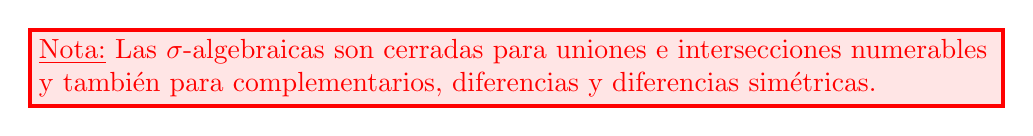
\begin{tikzpicture}
\node[red, draw=red, fill=red!10, line width=1.5, text width=\textwidth] {\underline{Nota:} Las $\sigma$-algebraicas son cerradas para uniones e intersecciones numerables y también para complementarios, diferencias y diferencias simétricas.};
\end{tikzpicture}

Sea $(\Omega,\mathcal{S},P)$ un espacio de probabilidad. Entonces:
\begin{enumerate}[label=\color{lightblue}\arabic*)]
	\item $P(\varnothing)=0$
	\item $P(A^c)=1-P(A)$
	\item Si $A,B\in\mathcal{S}$ tal que $A\cap B=\varnothing\longrightarrow P(A\cap B)=P(A)+P(B)$
	\item Si $A\subseteq B\longrightarrow P(B-A)=P(B)-P(A)$
	\item Si $A\subseteq B\longrightarrow P(A)\le P(B)$
	\item Si $A\in\mathcal{S}\longrightarrow P(A)\le1$
	\item $A,B\in\mathcal{S}\longrightarrow P(A\cup B)\le P(A)+ P(B)$
	\item $A,B\in\mathcal{S}\longrightarrow P(A\cup B)=P(A)+P(B)-P(A\cap B)$
	
	\begin{tikzpicture}
		\draw[fill=lightblue, opacity=0.5] (0,0) circle (1.5cm) ;
		\draw[fill=red, opacity=0.5] (2,0) circle (1.5cm) ;
		\draw (0,0) circle (1.5) node[above] {$A$};
		\draw (2,0) circle (1.5) node[above] {$B$};
	\end{tikzpicture}
	
	\item $A,B,C\in\mathcal{S}\longrightarrow P(A\cup B\cup C)=P(A)+P(B)+P(C)-P(A\cup B)-P(A\cap C)-P(B\cap C)+P(A\cap B\cap C)$
	
	\begin{tikzpicture}
		\fill[fill=lightblue, opacity=0.5] (0,0) circle (1.5);
		\fill[fill=red, opacity=0.5] (2,0) circle (1.5);
		\fill[fill=green, opacity=0.5] (1,-1.5) circle (1.5);
		\draw (0,0) circle (1.5) node[above] {$A$};
		\draw (2,0) circle (1.5) node[above] {$B$};
		\draw (1,-1.5) circle (1.5) node[below] {$C$};
	\end{tikzpicture}
\end{enumerate}
\begin{itemize}[label=\color{red}\textbullet, leftmargin=*]
	\item \color{lightblue}Propiedades (Función probabilidad)
\end{itemize}
\begin{tabular}{l:l}
	Proposición 1 & Proposición 2\\
	$P(\varnothing)=0$ & $P(A^c)=1-P(A)$\\
	Ax4\quad$P(\Omega)=1$ & $-$ Demostración:\\
	Ax6\quad$P(UA)=\sum P(A_i)$ & $\Omega=A\cup A^c\longrightarrow\lbb{P(\Omega)}{1}=P(A)+P(A^c)$\\
	$A-i\cap A_j=\varnothing\:\forall i\neq j$ & con $A$ y $A^c$ incompatibles\\
	$A_1=\Omega,\:A_2=A_3=\dots=\varnothing$ & \\
	$\begin{aligned}
		P(UA_i)&=P(\Omega)\\
		&=P(\Omega)+P(\varnothing)+\cdots+P(\varnothing)\\
		&\longrightarrow P(\varnothing)=0
	\end{aligned}$ & \\
	
\end{tabular}




